\section{Background and SCOC Process}

The core observing strategy for LSST is to cover large parts of the visible sky repeatedly every few days, in multiple bandpasses, over the course of ten years. The main survey (wide-fast-deep, WFD) has a design area of about 18,000 square degrees, to be observed under a wide range of conditions, giving faint co-added limiting magnitudes in ugrizy bandpasses. This survey will enable dark energy and dark matter cosmological studies and studies of the Milky Way structure with unprecedented precision; the same survey, when properly cadenced, can serve to open new windows into our understanding of transient sources and variable stars, and extend our knowledge of small bodies throughout the Solar System. The majority of available observing time will be spent on WFD; per the LSST Science Requirements Document (SRD, ls.st/srd) of the order 10\% of time will be spent on programs designed to maximize the science outcomes of LSST by exploring parameter space different from WFD. 

The basic necessary requirements to reach LSST science goals are listed in the SRD. A practical implementation of the observing strategy has more tunable parameters than specified in the SRD, thus leaving significant flexibility in the detailed cadence of observations. In order to maximize the science potential of LSST, the Rubin Observatory Construction and Early Operations teams have been collaborating with the LSST science community and other stakeholders from the start of the project, using a variety of approaches. They include a living collaborative document named the Community Observing Strategy Evaluation Paper, solicited Cadence White Papers and Cadence Notes, numerous performance metrics used to evaluate simulated surveys, and guidance from the LSST Science Advisory Committee (SAC) and SCOC. This pioneering process of community-focused experimental design is discussed in more detail by Bianco et al. (2021, arXiv/2108.01683). 

The current LSST baseline cadence strategy is an existence proof that the LSST dataset can be delivered as designed and advertised (for more details, see sections 2.1.5, 2.2.2 and 3.1 in the LSST overview paper, ls.st/lop). The simulations explored in the Fall 2020 Cadence Report (PSTN-051, https://pstn-051.lsst.io) offered variations on this survey strategy in an attempt to further enhance the baseline science yield from LSST. It is worth emphasizing that this optimization is essentially fine-tuning, rather than starting from scratch—anticipated gains for various metrics are closer to 10\% than, e.g., a factor of two. Based on the analysis to date, it is expected that science enhancements can be accomplished by varying at least some of the fundamental survey parameters, including: i) survey footprint and distribution of visits,  ii) exposure time per visit, iii) allocation of observing time per band (the distribution of visits between filters), and iv) time sampling (cadence) and dithers (on timescales from nightly to monthly to yearly). 

In order to facilitate the final phase of cadence optimization before the start of the 10-year Survey (anticipated in 2024), the SCOC was formed in 2020. The SCOC is an advisory body to the Rubin Observatory Operations Director and it will be a standing committee throughout the duration of LSST. Chaired by the Head of Science for LSST in operations, it will follow the progress of LSST and further optimize its observing strategy. The SCOC is responsible for optimizing the LSST cadence within the constraints imposed by the observing system, observing conditions, science drivers, and scientists invested in its mission and legacy. Its principal immediate tasks are to make specific recommendations for the initial survey strategy for the full 10-year survey, and to disseminate these recommendations via public reports and on-going engagement with the community. 

The remaining cadence optimization process prior to the start of operations is divided into two phases. The goal of phase 1 is to narrow the choice of the many different strategy options presented in the Fall 2020 LSST Cadence Optimization Report by making decisions about a few undecided optimization parameters, and by providing recommendations for the next generation of simulations, including the new baseline cadence. The draft phase 1 recommendation (this document) will be presented to stakeholders at the Project and Community Workshop in August 2021. After a dedicated workshop in November (Nov 16-17, 2021), when the SCOC hopes to receive feedback from all the stakeholders about the draft phase 1 recommendation, the recommendation will be finalized and broadly distributed before the end of calendar year 2021. 

The finalized document will serve as a guide for the concluding round of survey cadence simulations. The production of these simulations will begin prior to the November 2021 workshop and is expected to be completed during early calendar year 2022. Their analysis will inform the phase 2 survey strategy recommendation which will define the observing strategy for starting LSST. The phase 2 SCOC recommendation, and corresponding simulated and analyzed baseline survey, will be delivered to the Rubin Observatory Operations Director before the end of calendar year 2022. 

The main goal of phase 2 is to finalize the optimization of the new baseline cadence recommended in the phase 1 report, so that the adopted strategy can be implemented in the observatory  control system and tested during commissioning phase. It is expected that commissioning tests of the scheduling system will be undertaken during 2023, and that the operations phase will begin some time in 2024. In addition, phase 2 will include further optimization of cadences for the so-called Deep Drilling fields (DDFs), as well as modifications of adopted observing strategy to enhance early science goals (e.g., rapid production of templates for image differencing). 


\section{Phase 1 SCOC recommendations}

As a follow up to the Fall 2020 LSST Cadence Optimization Report and subsequent simulated surveys analysis by the LSST Science Collaborations, the SCOC solicited and received 39 Cadence Notes in April 2021 (available as ls.st/doc-37579). The call for Cadence Notes (ls.st/cadencenotes) aimed to fill additional gaps in metric coverage and get feedback on the existing large set of simulations, based on responses to seven specific questions. The summary SCOC  findings for each of these questions and resulting SCOC recommendations are listed below, followed by a detailed description of the next generation of survey simulations derived from these recommendations. 

Links:
\begin{itemize}
\item LSST Science Requirements Document,  (http://ls.st/SRD)
\item 2018 Cadence White Paper Submissions (https://www.lsst.org/submitted-whitepaper-2018, also available as a single download from http://ls.st/doc-30641)
\item Fall 2020 LSST Cadence Optimization Report (https://pstn-051.lsst.io)
\item 2020 Call for Cadence Notes (http://ls.st/cadencenotes)
\item 2021 Cadence Notes Submissions (https://www.lsst.org/content/survey-cadence-notes-2021, also available as a single download from http://ls.st/doc-37579)
\end{itemize}

{\it Q1: Are there any science drivers that would strongly argue for, or against, increasing the WFD footprint from 18,000 sq. deg. to 20,000 sq.deg.? Note that the resulting number of visits per pointing would drop by about 10\%. If available, please mention specific simulated cadences, and specific metrics, that support your answer. }
 
Findings and recommendations:

The responses to this question revealed that, rather than being simply an area vs visits tradeoff as posed, where that area is located in the sky is crucial to enabling the diverse LSST science goals. The SCOC has determined that various science-driven desiderata can be best satisfied by optimizing the area vs. the number of visits tradeoff separately in several different subregions of the main survey (WFD). The various requests by science communities can be best satisfied by considering the main survey to be composed of a low-dust-extinction survey area, a higher-extinction, high stellar density Galactic Bulge and Magellanic Clouds survey, and additionally ensuring coverage of the North Ecliptic Spur (NES), the remainder of the Galactic Plane and the remainder of the South Celestial Pole. The footprint for the low-dust-extinction part of the main survey will be motivated by the maximum acceptable value of the dust extinction, rather than by a simple boundary in Galactic coordinates as done originally. In addition, the low-dust-extinction survey area will be limited using two Declination limits (to be set later after a number of simulations with varied Dec limits, and perhaps more than one value of maximum acceptable dust extinction, are produced and analyzed). The cadence and footprint for the Galactic Bulge will also need to be modified/optimized. Once this new baseline simulation is produced, an alternative simulation where each visit will consist of a single exposure (a so-called snap, as opposed to two snaps in baseline cadence) will also be produced and analyzed.


{\it Q2: Assuming that current system performance estimates will hold up, we plan to utilize the additional observing time (which may be as much as 10\% of the survey observing time) for visits for the mini surveys and the DDFs (with an implicit assumption that the main WFD survey meeting SRD requirements will always be the first priority). What is the best scientific use of this time? }

Findings and recommendations:
 
The 10\% gain of the effective survey observing time is still hypothetical at this time. Potential
enhanced performance could be due to the delivered system throughput exceeding the nominal design value, an 8\% efficiency gain due to adopting 1x30s visits instead of 2x15s visits (which cannot be decided unless various tests prove satisfactory during commissioning), low solar activity resulting in darker night sky background, etc. However, it is also possible that the delivered performance will be lower than nominal, although this possibility has not been quantitatively explored yet.

There is no broad consensus for the 10\% usage between different science groups, although there is reasonable consistency within science groups; for example, cosmological drivers point to extending the low-extinction footprint, while Galactic science drivers argue for better Galactic plane and Magellanic cloud coverage. It is noteworthy that enhanced DDF coverage remains critical for better understanding of the WFD and thus simulations with more observing time dedicated to DDFs will be included in the next set of simulations. 

A number of "proposals" were submitted in response to the 2019 Cadence White Paper Call or the 2021 Cadence Note Call that were deemed "small" (so-called ‘micro-surveys’) because the implied use of observing time is at the level of a few \% or less. These micro-surveys are further divided into two groups; those requesting 0.3-3\% of the total observing time and those that requested < 0.3\% of the total observing time. The micro-surveys requesting above approximately 0.3\% of the total survey time include the following nine proposals that the SCOC recommends for simulation in phase 2:

\begin{table}[h]
\begin{tabular}{l | l}
             -- short description --             &                          -- obs. time -- \\
\hline
1) short twilight visits for near-Sun objects incl. NEOs      &   1-3\%  \\
2) ToO follow-up to ID counterparts to GW sources           &  1-2\% \\
3) mini-survey/DDF of Roman microlensing bulge field      &   ~2\% \\ 
4) Limited-visit survey of sky to Dec < +30                          &    1\% \\ 
5) static short exposure map of sky in ugrizy                     &  ~1\% \\
6) static to transient short exposure survey                         & 1-5\% \\
7) mini-survey of the virgo cluster to WFD depth                 &  ~1\% \\
8) deeper g-band imaging of ~ 10 local volume galaxies     & 0.3\% \\
9) high cadence survey of ~2 fields in SMC for microlenses&  0.3\% \\
\hline
\end{tabular}
\end{table}
  
Together, they correspond to about 12\% of observing time. The SCOC recommends to produce a family of simulations analogous to the baseline cadence where these proposals are individually, and to analyze them to assess the impact of their inclusion on various science performance metrics. Once this information is available, the final decision about these proposals, and the competing DDF cadences (currently allocated about 5\% of total observing time), can be included in phase 2 recommendations. It is noteworthy that there are no compelling reasons why any of these proposals must be attempted during the first year of operations, when the system performance might not be completely quantified. Therefore, this decision can also be revisited once a better understanding of the system is achieved.

It is worth noting that one of the micro-surveys listed above is related to ToO follow-up. While the special case to be investigated in the simulations is for follow-up to identify optical counterparts of gravitational wave sources (and this is the only compelling ToO case identified currently), in operations Rubin {\it does} expect to make some time available for Target of Opportunity observations, although the amount of time and policies for choosing these targets have yet to be decided in detail. General expectations are that this time would at most be a few percent of the total time available, that ToO proposals would be peer-reviewed, and that the alerts from ToO observations (at a minimum) would be distributed with the standard LSST alert stream.

There were also white papers and cadence notes submitted that requested less than ~0.3\% of the observing time, including requests of as little as 1 night of observing time (~0.03\%). Since the SCOC is not currently making recommendations for optimizing the survey at this level, these specific proposals will not be included in our phase 1 or 2 recommendations. However, the SCOC recommends that a small amount of observing time is allocated to such requests via a call for proposals to be issued after commissioning, when there is an improved quantitative understanding of the system performance. 

{\it Q3:  Are there any science drivers that would strongly argue for, or against, the proposal to change the u band exposure from 2x15 sec to 1x50 sec? }

Findings and recommendations:

Due to the dark sky in the u band, the impact of read-out noise is the largest in this band. Increasing the exposure time would improve the depth more rapidly than given by the canonical  square root of time scaling: if the u band exposure time changed from 2x15 sec to 1x50 sec, the single visit u band depth would improve by 0.5-0.6 mag\footnote{The increase of per-visit time (with overheads) from 39 sec (15+1+2+15+1+5, where 1 sec is for shutter motion, 2 sec for the first readout, with the second readout include in the typical slew time of 5 sec) to 56 sec (50+1+5), or by 44\%, would correspond effectively to an increase of observing time by almost a factor of 3 using the square root of time scaling of limiting magnitude (which is approximately correct in other bands). }

In the nominal per-band observing time allocation, the u band receives 56 visits out of 825 visits for all bands (about 7\% of total time). If the total time allocated to the u band were kept constant, the resulting number of visits would drop to 39. If instead the number of visits were kept constant, the additional 3-4\% of total observing time would have to be reallocated from other bands. For example, if 2\% of total observing time would be taken from the g and r bands, which are each allocated 22\% of total, the net relative effect for these bands would be about 10\% decrease in the number of visits (or equivalently about 0.08 single visit depth loss if the exposure time per visit was decreased by 2\% with the number of visits unchanged). 

The main science drivers for deeper u band data are photometric redshift estimates for galaxies and photometric metallicity estimates for stars earlier than MK spectral type K.  Deeper u band data are also beneficial for identifying quasars and for studying stellar flares.

The SCOC recommends that the u band visits include only a single snap. There should be two flavors of new baseline simulations: with 1x30 sec and 1x50 sec exposures, with the latter exploring both unchanged number of visits and unchanged total observing time in the u band. Aided by analysis of these simulations, the final choice will be left to phase 2 optimization. The key question will be whether additional time allocated to the u band with 1x50 sec exposures will have an unacceptable impact on observations in the g band (and possibly in the r band). We note that it is plausible that the ultimate choice could depend on Galactic latitude (differing between the low-extinction and higher-extinction portion of WFD).


{it Q4:  Are there any science drivers that would strongly argue for, or against, further changes in observing time allocation per band (e.g., skewed much more towards the blue or the red side of the spectrum)? }

Findings and recommendations:

There are no strong arguments for significantly changing the default per-band allocation of observing time. Of the submitted cadence notes that favored changing the filter allocation, there was a weak preference for improved bluer coverage, primarily in the g band (driven by studies involving star-forming galaxies, blue transients, and turn-off stars in the Milky Way). In order to quantitatively gauge the impact of changing the per band allocation, a small number of new simulations will be produced by modifying the new baseline to produce a larger number of visits in the g band for the main low-extinction survey. Detailed per-band optimization of specific regions, such as the North Ecliptic Spur and Galactic Plane/Bulge, will be left for phase 2 optimization of the adopted baseline strategy. 


{\it Q5:  Are there any science drivers that would strongly argue for, or against, obtaining two visits in a pair in the same (or different) filter? Or the benefits or drawbacks of dedicating  a portion of each night to obtaining a third (triplet) visit?   }

Findings and recommendations:

If two visits in a nightly pair are obtained in the same filter, we can reliably measure the brightness derivative on hourly time scales and quickly identify very exotic transients (those with dm/dt $>$ 1 mag/hr, e.g. gamma-ray burst afterglows). On the other hand, visits in different filters would enable color measurement for sources that vary on longer time scales, e.g., for supernovae and tidal disruption events. From the viewpoint of surveying efficiency, obtaining visits in the same filters increases efficiency by a few percent.

Based on the science-driven input provided, the SCOC recommends that pairs of visits be obtained with different filters to improve color constraints for sources that vary on time scales longer than several day (e.g. supernovae;  obtained mixed-filter nightly visit pairs provides a significant boost in their discovery rates). The detailed determination of which filters to use in each pair will be made during the next phase of survey strategy optimization, additional metrics tied to the related science return would be beneficial.  

In the previous round of simulations, visit pair time separation was varied (uniformly) from an interval of 22 minutes to intervals of 11, 33, 44 or 55 minutes; analysis shows that pairs of 33 minutes resulted in a higher survey efficiency, with no clear cost given current metrics and a potential gain in discovery of very distant solar system objects. Shorter visits were less efficient, longer intervals resulted in lower solar system object discovery and fewer pairs of visits. The SCOC thus recommends that the pair interval be changed to 33 minutes for the majority of the night. Simulations were also added which introduced a short-interval pair strategy during twilight (the interval is shorter because of the limited length of twilight and the desire to use different filter pairs during twilight than during the remainder of the night); as pairs generally offer the opportunity for variability or transient detection and also solar system object discovery, we recommend that pairs be executed during twilight with a shorter revisit interval (about 15 minutes). 

There are further modifications of the intra-night survey strategy that must also be considered: whether to obtain visits in triplets (adding a third visit in a filter matching an earlier visit, at a multi-hour time separation in order to provide that variability measurement) or to vary the time separation between pairs of visits. The SCOC recommends further investigation of the Presto-Color strategy (Bianco et al. White Paper) and greatly increased visit time separation (2-14 hours) (Bellm et al. Cadence Note) during these phase 2 simulations. 


{\it Q6:  Are there any science drivers that would strongly argue for, or against, the rolling cadence scenario? Or for or against varying the season length? Or for or against the AltSched N/S nightly pattern of visits? }

Findings and recommendations:

Our main recommendation is to continue to explore a rolling cadence: there are no strong arguments for rejecting this idea at this stage. The current—not fully optimized—implementation shows gains for at least some science metrics (most notably cosmological supernovae), but it is likely that further optimization is possible. However, the newest simulations (v1.7.1) were not addressed by all cadence notes, since they only recently became available, so the effects of a rolling cadence on a wide range of metrics is still uncertain.

To ensure a sufficient baseline for measuring high-quality proper motions and long-term variability, it is very unlikely that a rolling cadence would be implemented in the first ~ 1.5 years of the survey. Therefore we have more than 3 years before we have to deploy a rolling cadence strategy, allowing time for its detailed optimization. The next-generation baseline should utilize the current best rolling cadence implementation (see https://pstn-052.lsst.io), as simulated in the v1.7.1 release, and then continue optimizing it after the basic baseline strategy reaches some maturity. 

A task force including the Project Cadence Optimization Team and Science Collaboration members interested in rolling cadence (including but not limited to Cadence Notes authors Graham, Frohmeier, Hernitschek, Schwamb, Lochner, Bellm) will discuss efficient computation of metrics for the latest family of simulations, and potentially additional modified rolling cadence simulations; we are hopeful for more quantitative results by the time of November 2021 workshop.


{it Q7:  Are there any science drivers pushing for or against particular dithering patterns (either rotational dithers or translational dithers?)  }

Findings and recommendations:

We note that small camera rotations are executed in all sims in order to align the two visits from a pair, and visits to deep drilling fields. There are several metrics used in simulated cadence analysis that are sensitive to dithering and rotation angle uniformity (e.g. the Kuiper metric for the latter). 

There are no strong arguments for changing the implemented dithering pattern. We note that, however, it is possible that weak lensing systematics and analysis of low surface brightness features will require a different scheme but details will not be known until some commissioning data are in hand and analyzed. The Project needs to ensure that the tools needed to respond on an adequate time scale will be available by the start of commissioning. 
 


\section{Phase 2.0 Survey Simulations}

The next phase of survey strategy simulations consists of a limited set of survey strategy variations, evolving from the strategies tested in phase 1 (simulations in releases v1.5 to v1.7.1, described in PSTN-051). These simulations respond to the above SCOC findings and have been released as a group in v2.0. The main goals for remaining optimization, to be enabled by these (and possibly additional) simulations,  include:
\begin{itemize}
\item{Finalize survey footprint definitions (e.g. the exact Declination and dust extinction 
            limits for  the WFD region, exact definition of the Galactic bulge region, see below for 
            more details)}
\item{Decide which different filters should be used in pairs of visits}
\item{Decide the exposure duration and the number of visits in u band }
\item{Optimize further the rolling cadence implementation }
\item{Optimize further DDF cadences }
\end{itemize}

Once these goals are achieved, the SCOC will focus on modifications of adopted observing strategy to enhance early science from LSST (defined here as ``science prior to Data Release 1''). Below, we describe the updated baseline simulation, followed by descriptions of proposed v2.0 simulations. A more detailed description of the individual simulations available is online at \url{https://github.com/lsst-pst/survey_strategy/blob/main/fbs_2.0/SummaryInfo_v2.0.ipynb}, in the `SummaryInfo\_v2.0' notebook. 

\subsection{Baseline 2.0}

This simulation is an update of the baseline survey plan. Further numerical details will remain to be optimized, but there is a clear mandate to move to a new survey footprint. The updated footprint can generally be described as consisting of 
\begin{itemize}
\item A low-dust-extinction WFD region defined by north and south declination limits (approximately -72 deg. to +12 deg.) and an interstellar dust extinction upper limit (approximately E(B-V) = 0.2, or AV~0.6 mag)
\item Additional WFD-like regions defined by the locations of the Magellanic Clouds and an area of high stellar density in the Galactic bulge 
\item Lower level coverage of the remainder of the Galactic plane (GP) in $ugrizy$
\item Lower level coverage of the northern Ecliptic spur (NES) in $griz$ 
\item Lower level coverage of the remainder of the southern celestial pole (SCP) in $ugrizy$
\end{itemize}
This would comprise the ‘core’ survey footprint area, together with the five Deep Drilling fields (DDF), as shown in Figure~\ref{fig:baseline_v2.0_footprint}. The location of four of these DDFs was announced in 2011, while the adoption of the fifth DDF, which matches the Euclid Deep Field South, was recommended by the Survey Advisory Committee and agreed by the Operations Director in 2020, pending demonstration of feasibility. 

Visits in $grizy$ bands will be 2x15s, while visits in u band will be 1x30s. During twilight, visits will be taken in pairs with a 15 minute separation, instead of in singles as in the v1.X series baselines. During the remainder of the night, visits will be in pairs with approximately a 33 minute separation (with mixed filters between the pair), instead of about 22 minute separations as in the v1.X series baselines.

In the extragalactic (i.e., dust-extinction limited) WFD, a 2-band rolling cadence defined by declination will be implemented at approximately 90\% strength. The rolling cadence starts in approximately year 1.5 and ends at approximately year 8.5, to allow uninterrupted coverage of the entire sky in the first and last years of the survey. 

Some questions regarding the general baseline footprint which will be left for the next stage of survey strategy tuning include details of the survey footprint definition such as the exact Declination or dust extinction limits for the extragalactic WFD or the exact definition of the limits for the bulge WFD region, details of the filter balance in each region, and the definition of which different filters should be used in pairs of visits.


\begin{figure}[htbp]
\begin{center}
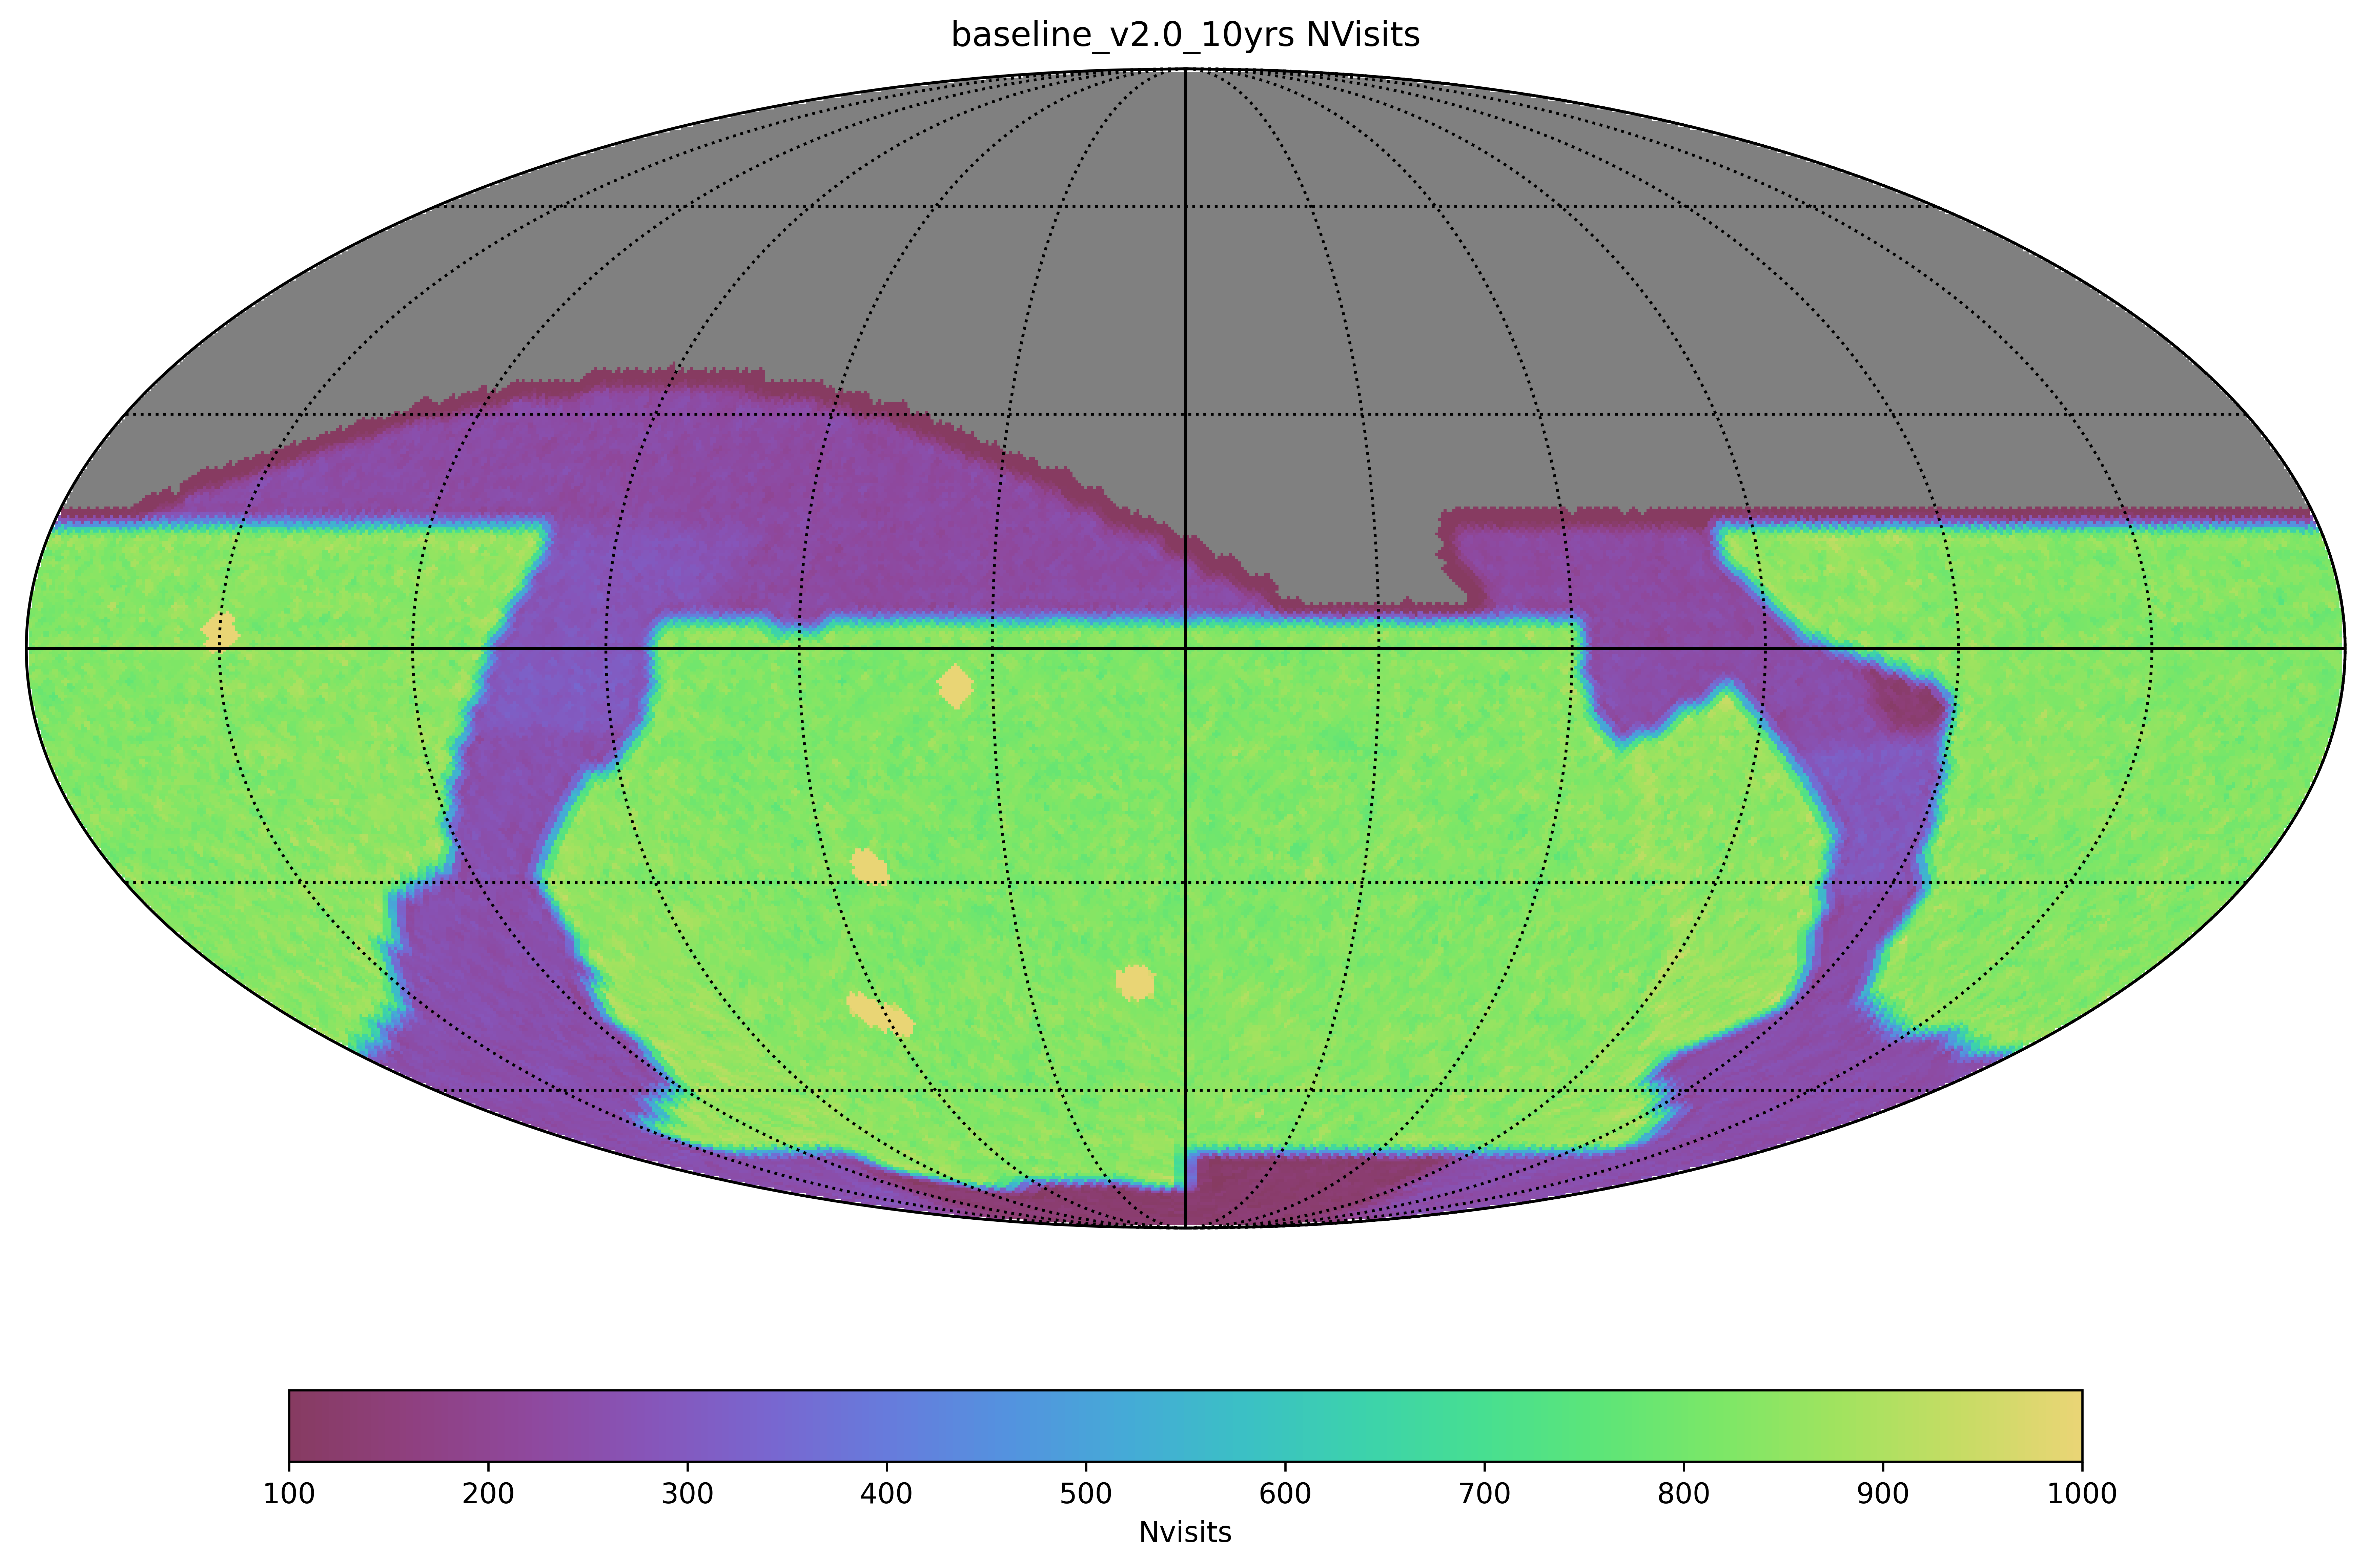
\includegraphics[width=0.8\textwidth]{baseline_v2_0_10yrs_Nvisits_HEAL_SkyMap}
\caption{Baseline v2.0 survey simulation, number of visits in all filters.}
\label{fig:baseline_v2.0_footprint}
\end{center}
\end{figure}



\subsection{Retro (comparison):}
These runs are intended to serve as a comparison point with previous simulations, to allow easier comparison of metrics between versions of the scheduler/simulation.
\begin{itemize} 
\item A classic ‘traditional’ survey footprint but with v2.0 settings - a halfway point between the classic footprint and the updated variations in the new simulations. This uses the standard ‘traditional’ survey footprint used in baselines from v1.5 to 1.7.1, 2x15s visits in grizy and 1x30s in u band, with a 2-band rolling cadence in WFD.
\item A classic ‘traditional’ v1.5-v1.7.1 survey footprint and v1.7.1 settings. This run would be directly comparable to baseline\_nexp2\_v1.7.1\_10yrs, but run with the newest version of the simulator. It uses the standard ‘traditional’ survey footprint used in baselines from v1.5 to 1.7.1, 2x15s visits in all bands, no rolling cadence.
\end{itemize}

\subsection{Rolling Cadence:}
These simulations add variations on the rolling cadence implementation. This is one of the largest areas that remains undecided with the new survey strategy. Many areas of science which may benefit from rolling cadence do not currently have quantitative metrics available. A metric related to SN detection indicates that a 2-band rolling cadence can significantly improve SN detection in the WFD, so a 2-band rolling cadence has been implemented in the low-extinction WFD region in the baseline. The impact of rolling cadence in the Galactic bulge or other mini-survey regions is not as clear, primarily due to a lack of relevant metrics. In addition to varying what regions and what fraction of the sky has rolling cadence, the strength of the rolling cadence is varied in this family. All simulations will use the updated baseline footprint 
and other v2.0 survey parameters (such as 1x30s visits in u band, 2x15s visits in grizy). 

The variations within this family include:
\begin{itemize}
\item No rolling cadence anywhere (in comparison to the 2-band rolling cadence in the baseline) % noroll 
\item 2-band rolling cadence in the low-dust WFD at varying strength and with variable start and end times % rolling
\item 3-band rolling cadence in the low-dust WFD at varying strength % rolling
\item 6-band rolling cadence in the low-dust WFD at varying strength % rolling_six
\item 2-band rolling cadence in the low-dust WFD and in the galactic bulge % rolling_bulge
\item 2-band rolling cadence in the low-dust WFD, in the bulge and the high extinction galactic plane % rolling_all_sky
\item 6-band rolling cadence in the galactic bulge % rolling_bulge_6
\end{itemize}
Note that in each of these rolling cadence simulations ‘2-band’ is referring to the fraction of the sky which is ‘active’ in rolling at any time. 2-band means ½ of the sky is rolling; 3-band means ⅓ of the sky is rolling. In each of these cases, the active sky area is further split into a North and South region, to better manage alert follow-up. 

\subsection{Longer u-band visits:}
The u-band visit time in the baseline is 1x30s, to avoid the penalty from read-noise for 2x15s snaps in u where this is most impactful. This family varies the visit time for u band to 1x50s, with two options on top of the baseline survey: 
\begin{itemize}
\item Longer u-band visit time, and approximately the same number of visits in u as in the baseline. This requires more survey time to be spent on u-band, so a few \% of time is removed from other bandpasses (altering the filter balance slightly). 
\item Longer u-band visit time, but the same relative amount of survey time. This reduces the number of visits in u-band accordingly.
\end{itemize} 

\subsection{More blue band visits:}
This family increases the time spent primarily in g (and u) for the low-extinction WFD. The u visits are kept at 1x30s: 
\begin{itemize}
\item Increase the fraction of visits in g from 9\% to 12\%, while keeping u at ~ 7\%
\item Increase the fraction of visits in g from 9\% to 11\% and increase u to ~ 8\%
\end{itemize}

\subsection{NES visits:}
The number of visits per pointing (and corresponding fraction of overall survey time) for the Northern Ecliptic Spur mini-survey is varied in this family of simulations. The overall survey footprint remains the same. The goal for the number of visits per pointing in the NES is approximately 30\% of the WFD in the baseline. This family varies the number of visits per pointing in the NES from 1 to 100\% relative to the WFD. 

\subsection{High dust extinction galactic plane visits: }
The number of visits per pointing (and the corresponding fraction of overall survey time) for the non-bulge regions of the Galactic plane (galactic plane mini-survey or `high dust extinction galactic plane') is varied in this family of simulations. The overall survey footprint remains the same. The goal number of visits per pointing in the non-bulge GP is approximately 27\% of WFD baseline visits per pointing in the baseline.  This family varies the number of visits per pointing in the non-bulge high extinction galactic plane from 1 to 100\% relative to the WFD.

\subsection{Deep Drilling fraction:}
The fraction of time spent on DD fields has been held constant at about 5\% evenly spread over the 5 DDF pointings in simulations v1.5 - 1.7.1. This family keeps the baseline survey strategy, but modifies the fraction of time spent on DDFs by a modest amount; the remainder of the survey footprint varies evenly up or down as the DDF fraction changes).

We note that the current implementation of DDF cadences is rather simplistic and requires further optimization, e.g., along the lines discussed in Lochner et al. Cadence Note. Our future DDF scheduling will use Mixed Integer Programming, making it easier to specify detailed cadences as well as try rolling cadence with the DDFs.

\subsection{Presto Color:}
The presto-color family could potentially cover a wide range of variations. The baseline survey strategy is modified so that triplets of visits are obtained in some nights, adding a third visit in a filter used earlier in the night in a pair. The triplet visit goal gap is varied per run, with values of 1.5, 2.0, 2.5, 3.0, 3.5, and 4.0 hours. As more visits are obtained in triplets, the overall number of visits per pointing or season length does not change; this drives the inter-night gap to slightly longer intervals; adding triplets for all visits throughout the survey is impractical for this reason, as it decreases for transients and variability. This is a slightly different implementation of “triplet visits per night” than in the third\_obs family provided in the v1.5 release, with a more precise timing interval for the third visit in the night and a higher fraction of visits in ‘triplets’.
\begin{itemize}
\item Triplets obtained with initial pair in g+r, r+i, or i+z. triplet gaps between 1.5 and 4 hours, triplets obtained either every night, or every other night
\item Triplets obtained with initial pair in g+i, r+z, or i+y. triplet gaps between 1.5 and 4 hours, triplets obtained either every night or every other night
\end{itemize}

\subsection{Long Gaps:}
These simulations are in response to the Bellm cadence note, which advocates for varying the time between pairs of visits starting after a few years (allowing the majority of solar system objects to be discovered in the first years of the survey, before switching to variable pair intervals). There are a wide variety of potential methods to implement these longer gaps between visits. For some of the simulations, we simply vary the interval between pairs from 2-7 hours (instead of the standard 33 minutes in the baseline). For some of the simulations, we keep the baseline pair but add a third visit at a long spacing (longer than in the Presto-Color family), between 2-14 hours.  A further variation is when or how often to run these long-interval pairs; throughout the entire survey or only starting after five years of standard surveying, and every night or every few nights. The options we have chosen to simulate here, hoping to span a reasonable range to show areas of future potential include:
\begin{itemize}
\item Variable visit spacing between 2-7 hours. The long spaced visits are obtained on every night up to every 7 nights.
\item Variable visit spacing between 2-7 hours. The long spaced visits are obtained on every night up to every 7 nights, but start after year 5.
\item Variable visit spacing between 2-7 hours where the initial visit is unpaired. The long spaced visits are obtained on every night up to every 7 nights. 
\item Variable visit spacing between 2-7 hours where the initial visit is unpaired. The long spaced visits are obtained on every night up to every 7 nights, but start after year 5.
\end{itemize}

\subsection{Variable Exposure Time:}
These simulations look at adjusting the exposure time for each visit to maintain more uniform individual image depth in each visit. This results in more (but shorter) exposures taking place in good conditions, and fewer (but longer) visits in poor conditions. Visit lengths are restricted to be between 20s and 100s. There are numerous ways that the `goal' depth could be set in practice, especially as this could vary with longer-term variations in the observing conditions; for this example, we defined the goal depth using the (known) expected depths from the weather simulations.

\subsection{Micro surveys: }
There are a large number of the so-called micro-surveys proposed in the 2018 white papers or 2021 cadence notes. They request up to ~3\% of LSST survey time for regions outside of the baseline footprint. There are at least 9 viable micro-surveys approved by the SAC or the SCOC detailed in those white papers, listed above, that are not addressed by the new recommended baseline survey. This family folds in each of these micro-surveys individually into the baseline survey strategy.  Some of the micro-surveys include multiple variations, such as the twilight NEO micro-survey. The SCOC does not recommend the simulation of sub-percent micro-surveys at the present time. The microsurveys include:
\begin{itemize}
\item Short twilight visits for near-Sun objects incl. NEOs (similar to the twilight\_NEO family in v1.7)
\item Annual 1-week survey of the Carina nebula and surrounding star forming regions
\item ToO follow-up to identify optical counterparts of gravitational wave sources
\item Micro survey of Roman microlensing bulge field
\item Addition of a northern stripe with a limited number of visits in ugrizy from the upper limit of the survey footprint to Dec=30
\item Single short (5s) exposure survey of the sky in ugrizy in year 1 for static sky calibration %short_exp
\item Multiple short exposures of the sky in ugrizy at a range of times for transient detection and static sky calibration %multi_short
\item Adding the Virgo Cluster to the WFD footprint
\item Deeper g-band imaging of 10 local volume galaxies
\item High cadence visits of 2 fields in the SMC for microlensing
\end{itemize}

The survey simulations outlined above are our best estimates of what these variations will encompass, with an approximation of the total number of simulations. These descriptions may be modified, and extended by additional simulations, when generating the set of v2.0 simulations. 
 
 More information about the actual runs simulated is available online at \url{https://github.com/lsst-pst/survey_strategy/blob/main/fbs_2.0/SummaryInfo_v2.0.ipynb}, in the 
 `SummaryInfo\_v2.0' notebook. 
 
\vskip 0.4in

\newcolumntype{L}{>{}p{0.7\columnwidth}}

\begin{table}[]
\begin{tabular}{l | L | l}
Family               & Brief Description       &    \# sims.   \\
\hline\hline
Baseline            & Updated survey footprint, 2x15s visits in grizy and 1x30s in u, 2-band rolling in WFD. &   1     \\
Retro comparison     & A comparison bridge point between v1.X and v2.0  & 2 \\
Rolling cadence      & Variations on the rolling cadence   & 13  \\
Longer u visits  & Extend  u-band visit time is extended to 1x50s    &    2 \\
More blue visits & Shift visits into bluer filters & 2 \\
NES visits & Vary the fraction of time spent on the NES & 14 \\
GP visits & Vary the fraction of time spent on the low-priority (non-bulge) regions of the GP & 14 \\
Deep Drilling fraction & Vary the fraction of time for DDFs & 2 \\
Presto Color & Add triplets of visits at varying times or fractions  & 12 \\
Long visit gaps & Vary the visit pair time between 2-10 hours after year 5  &  35 \\
Micro surveys & Add various micro-surveys from white papers  & 10 \\
\hline
 & Approximate total number of simulations &  120 \\
\hline
\end{tabular}
\end{table}\label{tab:shortlist}


\section{Metrics}

The SCOC strongly encourages the community to contribute science-motivated metrics, particularly to aid in evaluating the benefits or impacts of intra-night (presto-color and long visit gaps) and rolling cadence. The potential gains related to adding any of the micro-surveys (and thus removing time from the core survey) generally also need additional metrics. Metrics which bear on the survey footprint and its impact on evaluating Galactic structure would also be extremely helpful, for determining the extent of the WFD region in the Bulge and the coverage in the GP mini-survey. Many cadence notes were qualitative or did not have quantitative metrics ready that were fully incorporated into the Metric Analysis Framework (MAF). Without these metrics in MAF, they cannot be automatically run by the Rubin Observatory Scheduler Team when the new cadence simulations are available. The SCOC strongly encourages the community to liaise with the Rubin Observatory scheduler team to finalize metrics currently in development.  Metrics that are not incorporated into MAF before the end of 2021 risk not being included in the SCOC’s Phase 2 deliberations. 

\section{SCOC membership}

 Franz Bauer, Universidad Católica, Chile

 Sarah Brough, University of New South Wales 

 Renee Hlozek, University of Toronto

 Zeljko Ivezic, Rubin Observatory/University of Washington, chair

 Lynne Jones, Rubin Observatory (ex officio)

 Mansi Kasliwal, Caltech 

 Knut Olsen, NSF’s NOIRLab 

 Hiranya Peiris, University College London/Stockholm University

 Meg Schwamb, Queen's University Belfast

 Dan Scolnic, Duke University

 Colin Slater, University of Washington  

 Jay Strader, Michigan State University

 Peter Yoachim, Rubin Observatory/University of Washington (ex officio)

